% ===================================================================
%  PRESENTACIÓN PROYECTO GLOBAL INTEGRADOR — AyME 2026
%  Calderón, Joaquín — Castel, Francisco
%  Compilar con: pdflatex main_presentacion.tex
% ===================================================================
\documentclass[aspectratio=169,t]{beamer}

% ---------- Paquetes ----------
\usepackage[utf8]{inputenc}
\usepackage[T1]{fontenc}
\usepackage[spanish]{babel}
\usepackage{amsmath,amssymb,amsfonts,bm,mathtools}
\usepackage{graphicx}
\usepackage{xcolor}
\usepackage{booktabs}
\usepackage{array}
\usepackage{tabularx}
\usepackage{multirow}
\usepackage{textcomp}

% ---------- Tema minimalista (función > estética) ----------
\usetheme{default}
\setbeamertemplate{navigation symbols}{}    % sin barra de navegación

\definecolor{uncBlue}{RGB}{0,68,124}
\definecolor{uncGray}{RGB}{90,90,90}

\setbeamercolor{frametitle}{fg=uncBlue}
\setbeamerfont{frametitle}{series=\bfseries,size=\large}
\setbeamertemplate{frametitle}{%
  \vspace{2mm}\hspace{2mm}\insertframetitle\vspace{-2mm}%
}

% ---------- Footer azul con subsección a la izquierda y número a la derecha ----------
\setbeamercolor{footer_blue}{bg=uncBlue, fg=white}
\setbeamertemplate{footline}{%
  \leavevmode%
  \hbox{%
    \begin{beamercolorbox}[wd=\paperwidth, ht=2.8ex, dp=1.2ex, leftskip=3mm, rightskip=3mm]{footer_blue}%
      \scriptsize\insertsubsection\hfill\insertframenumber\,/\,\inserttotalframenumber%
    \end{beamercolorbox}%
  }%
}
\setbeamercolor{normal text}{fg=black}
\setbeamertemplate{itemize item}{\color{uncBlue}\textbullet}
\setbeamertemplate{itemize subitem}{\color{uncGray}--}

% ---------- Macros para tipos de slide ----------

% Slide-figura: título de sección + ayuda memoria + imagen al máximo
%   \figslide{TÍTULO DE SECCIÓN}{texto contextual/ayuda-memoria}{nombre_imagen.png}
\newcommand{\figslide}[3]{%
  \begin{frame}{#1}
    {\small\color{uncGray}#2}\par\vspace{2mm}
    \centering
    \includegraphics[width=0.98\textwidth,height=0.78\textheight,keepaspectratio]{imagenes/#3}
  \end{frame}
}

% Slide-ecuación destacada
\newcommand{\eqslide}[2]{%
  \begin{frame}{#1}
    \vspace{0.8cm}
    #2
    \vfill
  \end{frame}
}

% Slide de transición entre grandes secciones (card grande, solo título sin número)
\newcommand{\sectionslide}[1]{%
  \begin{frame}[plain]
    \vfill
    \centering
    {\Huge\bfseries\color{uncBlue} #1\par}
    \vfill
  \end{frame}
}

% ---------- Metadatos ----------
\title{Proyecto Global Integrador}
\subtitle{Control de Accionamiento de CA con Motor Sincrónico de Imanes Permanentes (PMSM)}
\author{Joaquín Calderón \and Francisco Castel}
\institute{UNCuyo --- Facultad de Ingeniería --- Ingeniería Mecatrónica\\
Espacio Curricular 311: Automática y Máquinas Eléctricas}
\date{2026}

\begin{document}

% ===================================================================
%  SLIDE 1 — PORTADA
% ===================================================================
\begin{frame}[plain]
  \centering
  \vspace{4mm}
  {\small UNIVERSIDAD NACIONAL DE CUYO\\
  Facultad de Ingeniería --- Ingeniería Mecatrónica\par}

  \vspace{3mm}
  {\small\color{uncGray} Espacio Curricular 311 --- Automática y Máquinas Eléctricas\par}

  \vspace{5mm}
  \rule{0.85\textwidth}{1pt}

  \vspace{5mm}
  {\huge\bfseries\color{uncBlue} Proyecto Global Integrador\par}

  \vspace{3mm}
  {\Large Control de Accionamiento de CA con\\Motor Sincrónico de Imanes Permanentes\par}

  \vspace{4mm}
  \rule{0.85\textwidth}{1pt}

  \vspace{3mm}
  {\large \textbf{Alumnos:}\par}
  \vspace{1mm}
  {\normalsize Joaquín Calderón \quad (Leg.\ 13839) \quad --- \quad Francisco Castel \quad (Leg.\ 13784)\par}

  \vspace{3mm}
  {\normalsize Mendoza, Argentina --- 2026\par}
\end{frame}

% ===================================================================
%  SLIDE 2 — ALCANCE Y OBJETIVOS
% ===================================================================
\begin{frame}{Alcance y objetivos del proyecto}
  {\small\color{uncGray}Sistema mecatrónico integrador: PMSM + inversor + reductor planetario + carga péndulo 1 GDL.}\par
  \vspace{4mm}

  \textbf{Objetivos:}
  \begin{itemize}
    \item Modelado matemático completo del accionamiento (NL, LPV y LTI equivalente).
    \item Análisis estructural (estabilidad, observabilidad, controlabilidad).
    \item Diseño de controlador en cascada (modulador de torque + PID externo + observador).
    \item Verificación de desempeño y especificaciones operativas.
    \item Discretización (Tustin) y codificación final (\textit{MATLAB Function}).
  \end{itemize}

  \vspace{3mm}
  \textbf{Componentes del sistema físico:}
  \begin{itemize}
    \item Máquina PMSM trifásica ($P_p=3$, $\lambda'_m=0{,}016$~Wb).
    \item Inversor trifásico desde CC ($V_{sl,max}=48$~Vca).
    \item Reductor planetario rígido $r=120{:}1$.
    \item Brazo manipulador 1~GDL, masa de carga útil variable $m_l\in[0;\,1{,}5]$~kg.
    \item Sensores: encoder en eje motor, 3 sensores de corriente de fase, RTD en bobinado.
  \end{itemize}
\end{frame}

% ===================================================================
%  SLIDE 3 — ÍNDICE / MAPA DEL TRABAJO
% ===================================================================
\begin{frame}{Mapa de la presentación}
  {\small\color{uncGray}Recorrido completo del trabajo desde la planta física hasta el código embebido.}\par
  \vspace{3mm}

  \begin{columns}[T]
    \column{0.48\textwidth}
    \textbf{Análisis a Lazo Abierto}
    \begin{enumerate}\small
      \item Modelado del subsistema mecánico equivalente.
      \item Modelo NL global de 6 estados en $qd0$.
      \item Linealización Jacobiana (LPV).
      \item Linealización por retroalimentación NL (LTI).
      \item Funciones de transferencia.
      \item Estabilidad, observabilidad y controlabilidad.
      \item Simulación dinámica NL vs LTI.
    \end{enumerate}

    \column{0.48\textwidth}
    \textbf{Controlador en Cascada}
    \begin{enumerate}\small\setcounter{enumi}{7}
      \item Modulador de torque (lazo interno).
      \item Controlador PID externo de movimiento.
      \item Observador reducido de orden 2.
      \item Simulación del sistema controlado.
      \item Verificación de límites operativos.
      \item Sensores e inversor no ideales.
      \item Discretización (Tustin) y codificación final.
      \item Conclusiones.
    \end{enumerate}
  \end{columns}
\end{frame}

% ===================================================================
%  BLOQUE B1 — PRESENTACIÓN DEL PROBLEMA
% ===================================================================

\subsection{Presentación del problema}
\sectionslide{Presentación del problema}

% -------------------------------------------------------------------
%  SLIDE 5 — Sistema bajo estudio (overview)
% -------------------------------------------------------------------
\figslide{Sistema bajo estudio}{%
Accionamiento eléctrico de 4 cuadrantes: Bus CC \textrightarrow{} Inversor trifásico \textrightarrow{} PMSM \textrightarrow{} Reductora planetaria ($r=120{:}1$) \textrightarrow{} Brazo manipulador 1 GDL. Tres conjuntos de sensores cierran la realimentación: corriente (CT), temperatura (RTD) y posición (encoder).%
}{diagrama_completo.png}

% -------------------------------------------------------------------
%  SLIDE 6 — Subsistemas y variables medidas
% -------------------------------------------------------------------
\figslide{Subsistemas y variables medidas}{%
\textbf{Eléctrico (potencia):} $V_{DC}$ alimenta al inversor 3\textphi{} (6 llaves IGBT/MOSFET, PWM).\quad
\textbf{Electromagnético + térmico:} estator en Y con neutro \emph{flotante}, $R_s(T_s^\circ)$ variable.\quad
\textbf{Mecánico:} reductora rígida $r=120{:}1$ + péndulo con carga útil $m_l$ y perturbación $T_{ld}$.\quad
\textbf{Sensores idealizados:} $i_{as},i_{bs},i_{cs}$ (CT), $T_s^\circ$ (RTD) y $\theta_m$ (encoder).%
}{diagrama_completo.png}

% -------------------------------------------------------------------
%  SLIDE 7 — Carga mecánica: brazo 1 GDL
% -------------------------------------------------------------------
\figslide{Carga mecánica: brazo manipulador rígido de 1 GDL}{%
Coordenada articular $q\equiv\theta_l$ referida al vertical hacia abajo (equilibrio estable). Sometido a gravedad $g=9{,}80665$~m/s$^2$ como perturbación externa constante. Masa de la barra $m=1{,}0$~kg, longitud $l_l=0{,}5$~m. Masa de carga útil variable $m_l\in[0;\,1{,}5]$~kg (no conocida a priori). Torque externo de contacto $T_{ld}\approx(0\pm 5)$~N$\cdot$m.%
}{brazo_1gdl.png}

% -------------------------------------------------------------------
%  SLIDE 8 — Especificaciones físicas
% -------------------------------------------------------------------
\begin{frame}{Especificaciones físicas del sistema}
{\small\color{uncGray}Parámetros nominales y rangos de variación admitidos en el diseño.}\par
\vspace{2mm}
\centering
\renewcommand{\arraystretch}{1.05}
\resizebox{\textwidth}{!}{%
\footnotesize
\begin{tabular}{|l|l|l||l|l|l|}
\hline
\textbf{Símb.} & \textbf{Descripción} & \textbf{Valor} & \textbf{Símb.} & \textbf{Descripción} & \textbf{Valor} \\
\hline
\multicolumn{3}{|c||}{\textbf{Mecánica (carga + transmisión)}} & \multicolumn{3}{c|}{\textbf{Eléctrica (PMSM)}} \\
\hline
$r$        & Relación de reducción         & $120{:}1$                     & $P_p$         & Pares de polos               & $3$ \\
$g$        & Aceleración gravedad          & $9{,}80665$~m/s$^2$           & $\lambda'_m$  & Flujo de imanes              & $0{,}016$~Wb \\
$m$        & Masa del brazo                & $1{,}0$~kg                    & $L_d$         & Inductancia eje directo      & $6{,}6$~mH \\
$l_{cm}$   & Long.\ centro de masa         & $0{,}25$~m                    & $L_q$         & Inductancia eje cuadratura   & $5{,}8$~mH \\
$l_l$      & Longitud al extremo           & $0{,}50$~m                    & $L_{ls}$      & Inductancia de dispersión    & $0{,}8$~mH \\
$m_l$      & Masa carga útil (variable)    & $0\dots 1{,}5$~kg             & $R_{sREF}$    & $R_s$ @ 20\,\textdegree{}C   & $1{,}02$~$\Omega$ \\
$b_l$      & Fricción articul.\ ($\pm 0{,}03$) & $0{,}1$~Nms/rad           & $J_m$         & Inercia rotor (m+caja)       & $14{\times}10^{-6}$~kg\,m$^2$ \\
$T_{ld}$   & Perturbación de contacto      & $0\pm 5$~N$\cdot$m            & $b_m$         & Fricción rotor (m+caja)      & $15{\times}10^{-6}$~Nms/rad \\
\hline
\multicolumn{6}{|c|}{\textbf{Térmico}} \\
\hline
\multicolumn{2}{|l|}{$C_{ts}$ — Capacitancia térmica del estator}              & $0{,}818$~W/(\textdegree{}C/s) &
\multicolumn{2}{l|}{$\alpha_{Cu}$ — Coef.\ térmico del cobre}                  & $3{,}9{\times}10^{-3}$~/\textdegree{}C \\
\multicolumn{2}{|l|}{$R_{ts\text{-}amb}$ — Resistencia térmica al ambiente}    & $146{,}7$~\textdegree{}C/W      &
\multicolumn{2}{l|}{$\tau_{ts\text{-}amb}=R_{ts\text{-}amb}\cdot C_{ts}$}      & $\approx 120$~s \\
\hline
\end{tabular}%
}
\end{frame}

% -------------------------------------------------------------------
%  SLIDE 9 — Especificaciones operativas y límites
% -------------------------------------------------------------------
\begin{frame}{Especificaciones operativas y límites a respetar}
{\small\color{uncGray}Restricciones impuestas por la caja reductora, el motor y el inversor. Determinarán el espacio de operación admisible.}\par
\vspace{2mm}
\centering
\renewcommand{\arraystretch}{1.2}
\resizebox{\textwidth}{!}{%
\footnotesize
\begin{tabular}{|l|l|c|l|}
\hline
\textbf{Componente} & \textbf{Magnitud} & \textbf{Valor} & \textbf{Observación} \\
\hline
\multirow{2}{*}{Caja reductora (salida)}
   & Velocidad nominal $n_{l,nom}$                       & $60$~rpm ($\omega_{l,nom}=6{,}28$~rad/s)       & Régimen continuo \\
   & Torque nominal/pico $T_{q,nom}\,/\,T_{q,max}$       & $17{,}0\,/\,45{,}0$~N$\cdot$m                  & Pico: aceleración corta \\
\hline
\multirow{4}{*}{Motor PMSM (estator)}
   & Velocidad nominal rotor $n_{m,nom}$                 & $6600$~rpm ($\omega_{m,nom}=691{,}15$~rad/s)   & \\
   & Tensión nominal línea $V_{sl,nom}$                  & $30$~Vca rms                                   & $V_{sf,nom}=V_{sl,nom}/\sqrt{3}$ \\
   & Corriente nominal/pico $I_{s,nom}\,/\,I_{s,max}$    & $0{,}4\,/\,2{,}0$~Aca rms                      & Pico: corta duración \\
   & Temperatura máxima bobinado $T_{s,max}^\circ$       & $115$~\textdegree{}C                           & RTD de protección \\
\hline
\multirow{2}{*}{Inversor trifásico}
   & Tensión máxima línea $V_{sl,max}$                   & $48$~Vca rms                                   & Saturación dura \\
   & Frecuencia eléctrica $f_e$                          & $[-330,\,0,\,+330]$~Hz                         & Signo $\Rightarrow$ sentido de giro \\
\hline
\multirow{2}{*}{Perturbaciones externas}
   & Torque de contacto $T_{ld}$                         & $0\pm 5{,}0$~N$\cdot$m                         & Asumido escalón \\
   & Temperatura ambiente $T_{amb}^\circ$                & $[-15,\,+40]$~\textdegree{}C                   & Cuasi-constante \\
\hline
\end{tabular}%
}
\end{frame}

% ===================================================================
%  BLOQUE B2 — SUBSISTEMA MECÁNICO EQUIVALENTE
% ===================================================================

\subsection{Subsistema mecánico equivalente}
\sectionslide{Subsistema mecánico equivalente}

% -------------------------------------------------------------------
%  SLIDE 11 — Modelado de la carga mecánica
% -------------------------------------------------------------------
\begin{frame}{Modelado de la carga mecánica (péndulo 1 GDL)}
{\small\color{uncGray}Brazo manipulador rígido de 1 g.d.l., eje horizontal fijo a la base, sometido a gravedad $g$ como perturbación externa constante y a un torque de contacto $T_{ld}(t)$ tratado como escalón.}\par
\vspace{3mm}

\textbf{Ecuación dinámica:}
\begin{equation*}
J_l\,\dot{\omega}_l(t) = T_q(t) - b_l\,\omega_l(t) - T_l(t)
\end{equation*}

\textbf{Torque de carga} = gravitatorio + perturbación:
\begin{equation*}
T_l(t) = g\,k_l\,\sin\!\big(\theta_l(t)\big) + T_{ld}(t)
\end{equation*}

\textbf{Parámetros equivalentes referidos al eje de salida del reductor:}
\begin{align*}
J_l &= m\,l_{cm}^2 + J_{cm} + m_l\,l_l^2 \;=\; 0{,}0833 + [0\dots 0{,}375]\;\;\text{kg}\cdot\text{m}^2 \\
k_l &= m\,l_{cm} + m_l\,l_l \;=\; 0{,}25 + [0\dots 0{,}75]\;\;\text{kg}\cdot\text{m}
\end{align*}

\vspace{1mm}
{\small Relación cinemática: $\dot{\theta}_l(t)=\omega_l(t)$.}
\end{frame}

% -------------------------------------------------------------------
%  SLIDE 12 — Tren de transmisión rígido
% -------------------------------------------------------------------
\begin{frame}{Tren de transmisión rígido}
{\small\color{uncGray}Caja reductora reversible con engranajes planetarios, relación $r=120{:}1$. Bajo las hipótesis adoptadas, todos los términos disipativos e inerciales internos se reflejan al eje del motor.}\par
\vspace{4mm}

\textbf{Hipótesis del modelo equivalente:}
\begin{itemize}
\item Ausencia de \textit{backlash} (juego mecánico nulo).
\item Ausencia de elasticidad torsional (acoplamiento rígido ideal).
\item Inercia y fricción internas ya incluidas en $J_m$ y $b_m$.
\end{itemize}

\vspace{4mm}
\textbf{Relaciones de transformación motor $\leftrightarrow$ carga:}
\begin{equation*}
\omega_l(t) = \frac{1}{r}\,\omega_m(t)
\qquad\qquad
T_q(t) = r\,T_d(t)
\qquad\qquad
\theta_l(t) = \frac{1}{r}\,\theta_m(t)
\end{equation*}

\vspace{4mm}
{\small La rigidez del tren permite tratar carga, transmisión y rotor como una única unidad mecánica de 1~GDL, simplificando el modelo a un único subsistema mecánico equivalente.}
\end{frame}

% -------------------------------------------------------------------
%  SLIDE 13 — Subsistema mecánico del rotor
% -------------------------------------------------------------------
\begin{frame}{Subsistema mecánico del rotor de la PMSM}
{\small\color{uncGray}Balance de cuplas del rotor referido al estator estacionario. La inercia y fricción internas de la caja reductora ya están reflejadas en $J_m$ y $b_m$ por hipótesis de transmisión rígida.}\par
\vspace{4mm}

\textbf{Ecuación dinámica del rotor (balance de cuplas):}
\begin{equation*}
J_m\,\dot{\omega}_m(t) = T_m(t) - b_m\,\omega_m(t) - T_d(t)
\end{equation*}

\textbf{Cinemática del rotor:}
\begin{equation*}
\dot{\theta}_m(t) = \omega_m(t)
\end{equation*}

\textbf{Variables del balance:}
\begin{itemize}
\item $T_m(t)$: torque electromagnético entregado por las corrientes del estator vía la interacción con el flujo de los imanes (se deriva en la sección electromagnética: $T_m = \tfrac{3}{2}P_p\lambda'_m i_{qs}^r + \tfrac{3}{2}P_p(L_d-L_q)i_{ds}^r i_{qs}^r$).
\item $T_d(t)$: cupla de reacción transferida al tren de transmisión, despejada en la combinación algebraica con el péndulo (slide siguiente).
\item $J_m,\,b_m$: parámetros nominales del conjunto rotor + caja (ver tabla de especificaciones físicas).
\end{itemize}
\end{frame}

% -------------------------------------------------------------------
%  SLIDE 14 — Combinación algebraica
% -------------------------------------------------------------------
\begin{frame}{Combinación: derivación del modelo equivalente}
{\small\color{uncGray}Sustituyendo las relaciones del tren rígido en la ecuación del péndulo y combinando con la ecuación del rotor, la variable intermedia $T_d$ se elimina algebraicamente.}\par
\vspace{2mm}

\textbf{Paso 1.} Sustituyendo $\omega_l = \omega_m/r$ y $T_q = r\,T_d$ en la ecuación del péndulo:
\begin{equation*}
\tfrac{J_l}{r}\,\dot{\omega}_m(t) = r\,T_d(t) - \tfrac{b_l}{r}\,\omega_m(t) - T_l(t)
\end{equation*}

\textbf{Paso 2.} Despejando $T_d$ y usando $T_l = g\,k_l\sin(\theta_m/r)+T_{ld}$:
\begin{equation*}
T_d(t) = \tfrac{J_l}{r^2}\,\dot{\omega}_m + \tfrac{b_l}{r^2}\,\omega_m + \tfrac{1}{r}\!\left[g\,k_l\,\sin\!\big(\tfrac{\theta_m}{r}\big) + T_{ld}(t)\right]
\end{equation*}

\textbf{Paso 3.} Reemplazando $T_d$ en la ecuación del rotor ($J_m\dot{\omega}_m=T_m-b_m\omega_m-T_d$) y agrupando términos en $\dot{\omega}_m$ y $\omega_m$ se obtiene la ecuación equivalente compactada (siguiente slide).
\end{frame}

% -------------------------------------------------------------------
%  SLIDE 15 — Modelo equivalente al eje del motor
% -------------------------------------------------------------------
\begin{frame}{Modelo mecánico equivalente al eje del motor}
{\small\color{uncGray}Ecuación única de balance de cuplas que reúne motor, caja reductora y carga. La no linealidad gravitacional queda como término $\sin(\theta_m/r)$.}\par
\vspace{8mm}

\begin{equation*}
\boxed{\;\;
J_{eq}\,\dot{\omega}_m(t) = T_m(t) - b_{eq}\,\omega_m(t) - \tfrac{1}{r}\!\left[g\,k_l\,\sin\!\big(\tfrac{\theta_m(t)}{r}\big) + T_{ld}(t)\right]
\;\;}
\end{equation*}

\vspace{8mm}
\textbf{¿Por qué se puede compactar?}
\begin{itemize}
\item La rigidez del tren ($r=120{:}1$) permite reflejar $J_l$ y $b_l$ al eje del motor con factor $1/r^2$.
\item Al desaparecer $T_d$ el sistema mecánico se reduce de 2 EDOs a 1 (orden 2 con $\theta_m,\omega_m$).
\item La perturbación gravitatoria queda como término no lineal $\sin(\theta_m/r)$.
\end{itemize}
\end{frame}

% -------------------------------------------------------------------
%  SLIDE 16 — Parámetros equivalentes
% -------------------------------------------------------------------
\begin{frame}{Parámetros mecánicos equivalentes (valores nominales)}
{\small\color{uncGray}Definiciones y evaluación numérica para el caso sin carga útil ($m_l=0$) y para la carga útil máxima ($m_l=1{,}5$~kg). Se observa la dilución del acoplamiento mecánico por el factor $r^2$.}\par
\vspace{3mm}

\textbf{Definiciones:}
\begin{equation*}
J_{eq} = J_m + \frac{J_l}{r^2}
\qquad\qquad
b_{eq} = b_m + \frac{b_l}{r^2}
\end{equation*}

\vspace{4mm}
\textbf{Evaluación numérica con $r=120$:}\par
\vspace{2mm}
\centering
\renewcommand{\arraystretch}{1.25}
\begin{tabular}{|l|c|c|c|}
\hline
\textbf{Magnitud} & \textbf{Mínima ($m_l=0$)} & \textbf{Máxima ($m_l=1{,}5$)} & \textbf{Unidad} \\
\hline
$J_l$    & $0{,}0833$              & $0{,}4583$              & kg$\cdot$m$^2$ \\
$k_l$    & $0{,}25$                & $1{,}375$               & kg$\cdot$m \\
$J_{eq}$ & $1{,}98\times 10^{-5}$  & $4{,}58\times 10^{-5}$  & kg$\cdot$m$^2$ \\
$b_{eq}$ & $2{,}19\times 10^{-5}$  & $2{,}19\times 10^{-5}$  & Nms/rad \\
\hline
\end{tabular}

\vspace{3mm}
{\small La incertidumbre $b_l\pm 0{,}03$ aporta $\pm 2{,}08{\times}10^{-6}$~Nms/rad a $b_{eq}$ (~$\sim 10\%$).}
\end{frame}

% -------------------------------------------------------------------
%  SLIDE 17 — Ecuaciones de estado del subsistema mecánico
% -------------------------------------------------------------------
\begin{frame}{Ecuaciones de estado del subsistema mecánico}
{\small\color{uncGray}Estado: $\bm{x}_{mec}=[\theta_m,\omega_m]^T$. Entradas: $T_m$ (manipulada) y $T_{ld}$ (perturbación). Salida medida: posición angular $\theta_m$.}\par
\vspace{2mm}

\textbf{Forma escalar:}
\begin{equation*}
\begin{cases}
\dot{\theta}_m(t) = \omega_m(t) \\[4pt]
\dot{\omega}_m(t) = -\dfrac{b_{eq}}{J_{eq}}\,\omega_m(t) -\dfrac{g\,k_l}{J_{eq}\,r}\,\sin\!\big(\tfrac{\theta_m(t)}{r}\big) +\dfrac{1}{J_{eq}}\,T_m(t) -\dfrac{1}{J_{eq}\,r}\,T_{ld}(t) \\[6pt]
y(t) = \theta_m(t)
\end{cases}
\end{equation*}

\vspace{2mm}
\textbf{Forma matricial} --- el término $\sin(\cdot)$ impide escribir $\dot{\bm{x}}=\bm{A}\bm{x}+\bm{B}\bm{u}$ estándar; el sistema es \textbf{no lineal}:
\begin{equation*}
\begin{bmatrix}\dot{\theta}_m \\ \dot{\omega}_m\end{bmatrix} =
\underbrace{\begin{bmatrix}\omega_m \\[2pt] -\tfrac{g\,k_l}{J_{eq}\,r}\sin\!\big(\tfrac{\theta_m}{r}\big) -\tfrac{b_{eq}}{J_{eq}}\,\omega_m\end{bmatrix}}_{\bm{f}(\bm{x})}
+
\underbrace{\begin{bmatrix}0 & 0 \\[2pt] \tfrac{1}{J_{eq}} & -\tfrac{1}{J_{eq}\,r}\end{bmatrix}}_{\bm{B}}
\begin{bmatrix}T_m(t) \\ T_{ld}(t)\end{bmatrix}
\end{equation*}
\end{frame}

% ===================================================================
%  BLOQUE B3 — SUBSISTEMA ELECTROMAGNÉTICO QD0 + PARK
% ===================================================================

\subsection{Subsistema electromagnético en coordenadas qd0}
\sectionslide{Subsistema electromagnético en coordenadas rotóricas $qd0$}

% -------------------------------------------------------------------
%  SLIDE 19 — Marco de referencia rotórico (concepto y cinemática)
% -------------------------------------------------------------------
\begin{frame}{Marco de referencia rotórico ($qd0$)}
{\small\color{uncGray}La transformación de Park proyecta las variables trifásicas $abc$ (marco estacionario) sobre un marco fijo al rotor, sincrónico con éste en régimen estacionario. En operación equilibrada las variables resultantes son cuasi-DC.}\par
\vspace{3mm}

\textbf{Posición angular del rotor en coordenadas eléctricas:}
\begin{equation*}
\theta_r(t) \equiv P_p\,\theta_m(t)
\qquad\Longleftrightarrow\qquad
\omega_r(t) = P_p\,\omega_m(t)
\end{equation*}

\textbf{Relación cinemática (consistencia ángulo $\leftrightarrow$ velocidad):}
\begin{equation*}
\frac{d\theta_r(t)}{dt} \equiv \omega_r(t)
\qquad\Longleftrightarrow\qquad
\theta_r(t) = \int_{t_0}^{t} \omega_r(\xi)\,d\xi + \theta_r(t_0)
\end{equation*}

\vspace{2mm}
\textbf{Ventajas del marco rotórico para el modelado:}
\begin{itemize}\small
\item Las corrientes y tensiones $abc$ sinusoidales se transforman en componentes cuasi-DC en régimen.
\item El acoplamiento entre el flujo de los imanes (eje $d$) y la cupla útil (eje $q$) queda explícito.
\item Permite formular el control vectorial: separar la dinámica de flujo de la de torque.
\end{itemize}
\end{frame}

% -------------------------------------------------------------------
%  SLIDE 20 — Tensiones trifásicas en abc (entregadas por el inversor)
% -------------------------------------------------------------------
\begin{frame}{Tensiones trifásicas referidas al estator ($abc$)}
{\small\color{uncGray}El inversor sintetiza un sistema trifásico balanceado de tensiones desfasadas $120^\circ$ entre fases. $\theta_{ev}(t)$ es la posición angular eléctrica del fundamental del estator (referida a la tensión $v_{as}$).}\par
\vspace{4mm}

\textbf{Componentes de fase del estator:}
\begin{align*}
v_{as}(t) &= V_m\,\cos\!\big(\theta_{ev}(t)\big) \\
v_{bs}(t) &= V_m\,\cos\!\big(\theta_{ev}(t) - \tfrac{2\pi}{3}\big) \\
v_{cs}(t) &= V_m\,\cos\!\big(\theta_{ev}(t) + \tfrac{2\pi}{3}\big)
\end{align*}

\textbf{Vector trifásico de tensiones del estator:}
\begin{equation*}
\bm{\mathrm{v}}_{abcs}(t) \equiv \big[\,v_{as}(t),\;v_{bs}(t),\;v_{cs}(t)\,\big]^T
\end{equation*}

\textbf{Frecuencia eléctrica del estator (variable manipulable por el inversor):}
\begin{equation*}
\omega_e(t) \equiv 2\pi f_e(t) = \frac{d\theta_{ev}(t)}{dt}
\qquad\text{con}\quad f_e\in[-330,\,0,\,+330]\;\text{Hz}
\end{equation*}

{\small El signo de $f_e$ define la secuencia $abc$/$acb$ y por ende el sentido de giro del campo rotante.}
\end{frame}

% -------------------------------------------------------------------
%  SLIDE 21 — Matriz de Park K_s
% -------------------------------------------------------------------
\begin{frame}{Transformación de Park: matriz $K_s(\theta_r)$}
{\small\color{uncGray}Operador lineal que proyecta cualquier vector trifásico $\bm{x}_{abcs}$ sobre el marco rotórico $\bm{x}^{r}_{qd0s}$. La matriz $K_s$ depende explícitamente de la posición eléctrica del rotor $\theta_r$.}\par
\vspace{3mm}

\textbf{Relación directa $abc \rightarrow qd0$:}
\begin{equation*}
\bm{x}^{r}_{qd0s}(t) = K_s\!\big(\theta_r(t)\big)\;\bm{x}_{abcs}(t)
\qquad\text{con}\qquad \bm{x}\in\{\bm{v},\,\bm{i},\,\bm{\lambda}\}
\end{equation*}

\textbf{Matriz de Park (convención estándar de Krause):}
\begin{equation*}
K_s(\theta_r) = \frac{2}{3}
\begin{bmatrix}
\cos\theta_r & \cos\!\big(\theta_r-\tfrac{2\pi}{3}\big) & \cos\!\big(\theta_r+\tfrac{2\pi}{3}\big) \\[4pt]
\sin\theta_r & \sin\!\big(\theta_r-\tfrac{2\pi}{3}\big) & \sin\!\big(\theta_r+\tfrac{2\pi}{3}\big) \\[4pt]
\tfrac{1}{2} & \tfrac{1}{2} & \tfrac{1}{2}
\end{bmatrix}
\end{equation*}

\textbf{Transformación inversa $qd0\rightarrow abc$:}
\begin{equation*}
\bm{x}_{abcs}(t) = K_s^{-1}\!\big(\theta_r(t)\big)\;\bm{x}^{r}_{qd0s}(t)
\end{equation*}

{\small El factor $2/3$ se elige para que las amplitudes pico se preserven al transformar (convención \emph{amplitud-invariante}).}
\end{frame}

% -------------------------------------------------------------------
%  SLIDE 22 — Ecuaciones de tensión en qd0 (rotor)
% -------------------------------------------------------------------
\begin{frame}{Tensiones de estator referidas al rotor ($qd0$)}
{\small\color{uncGray}Aplicando $K_s$ a las ecuaciones del estator equilibrado y simétrico, se obtienen tres ecuaciones desacopladas en los términos puramente inductivos, pero acopladas a través de la velocidad del rotor.}\par
\vspace{3mm}

\textbf{Eje cuadratura ($q$):}
\begin{equation*}
v^{r}_{qs}(t) = R_s\!\big(T_s^\circ\big)\,i^{r}_{qs}(t) + L_q\,\frac{d i^{r}_{qs}(t)}{dt} + \big[\,\lambda'_m + L_d\,i^{r}_{ds}(t)\,\big]\,\omega_r(t)
\end{equation*}

\textbf{Eje directo ($d$):}
\begin{equation*}
v^{r}_{ds}(t) = R_s\!\big(T_s^\circ\big)\,i^{r}_{ds}(t) + L_d\,\frac{d i^{r}_{ds}(t)}{dt} - L_q\,i^{r}_{qs}(t)\,\omega_r(t)
\end{equation*}

\textbf{Eje homopolar ($0$):}
\begin{equation*}
v^{r}_{0s}(t) = R_s\!\big(T_s^\circ\big)\,i^{r}_{0s}(t) + L_{ls}\,\frac{d i^{r}_{0s}(t)}{dt}
\end{equation*}

\vspace{1mm}
{\small \textbf{Estructura común:} caída resistiva + caída inductiva + acoplamiento de velocidad (FCEM de imanes y/o acoplamiento cruzado $qd$).}
\end{frame}

% -------------------------------------------------------------------
%  SLIDE 23 — Identificación de los acoplamientos
% -------------------------------------------------------------------
\begin{frame}{Identificación física de los acoplamientos}
{\small\color{uncGray}Cada término de las ecuaciones de tensión tiene una interpretación física concreta. Estos acoplamientos son justamente los que el modulador de torque (sección 5.2.1) cancelará por retroalimentación para linealizar la dinámica.}\par
\vspace{4mm}

\textbf{Eje $q$:}
\begin{equation*}
v^{r}_{qs} = \underbrace{R_s\,i^{r}_{qs}}_{\text{disipación}} + \underbrace{L_q\tfrac{di^{r}_{qs}}{dt}}_{\text{inductivo}} + \underbrace{\lambda'_m\,\omega_r}_{\text{FCEM de imanes}} + \underbrace{L_d\,i^{r}_{ds}\,\omega_r}_{\text{acopl.\ cruzado $d\to q$}}
\end{equation*}

\textbf{Eje $d$:}
\begin{equation*}
v^{r}_{ds} = \underbrace{R_s\,i^{r}_{ds}}_{\text{disipación}} + \underbrace{L_d\tfrac{di^{r}_{ds}}{dt}}_{\text{inductivo}} \underbrace{-\,L_q\,i^{r}_{qs}\,\omega_r}_{\text{acopl.\ cruzado $q\to d$}}
\end{equation*}

\vspace{2mm}
\textbf{Observaciones clave:}
\begin{itemize}\small
\item $R_s$ depende de la temperatura $T_s^\circ(t) \;\Rightarrow$ acoplamiento con el subsistema térmico.
\item Los términos $\propto \omega_r$ acoplan dinámicamente la dinámica eléctrica con la mecánica.
\item Si se impone $i^{r}_{ds}\equiv 0$ (\textbf{control vectorial con campo orientado}), el acoplamiento cruzado del eje $q$ se reduce a $\lambda'_m\omega_r$ y la dinámica de $i^{r}_{qs}$ se vuelve lineal de primer orden.
\end{itemize}
\end{frame}

% -------------------------------------------------------------------
%  SLIDE 24 — Torque electromagnético
% -------------------------------------------------------------------
\begin{frame}{Torque electromagnético: imanes + reluctancia}
{\small\color{uncGray}La cupla entregada por la PMSM tiene dos contribuciones independientes: la interacción del flujo de los imanes con la corriente en cuadratura, y el torque de reluctancia debido a la asimetría magnética del rotor ($L_d\neq L_q$).}\par
\vspace{8mm}

\begin{equation*}
\boxed{\;\;
T_m(t) = \underbrace{\tfrac{3}{2}\,P_p\,\lambda'_m\,i^{r}_{qs}(t)}_{\text{torque de imanes}} \;+\; \underbrace{\tfrac{3}{2}\,P_p\,(L_d - L_q)\,i^{r}_{ds}(t)\,i^{r}_{qs}(t)}_{\text{torque de reluctancia}}
\;\;}
\end{equation*}

\vspace{8mm}
\textbf{Implicaciones para el control:}
\begin{itemize}\small
\item Con polos no salientes ideales ($L_d=L_q$): subsiste solo el torque por imanes, lineal en $i^{r}_{qs}$.
\item En esta máquina $L_d>L_q$ (rotor de polos ligeramente salientes), por lo que $i^{r}_{ds}\neq 0$ aporta torque de reluctancia.
\item \textbf{Estrategia base:} forzar $i^{r}_{ds}\equiv 0 \;\Rightarrow\; T_m = \tfrac{3}{2}P_p\lambda'_m\,i^{r}_{qs}$ (lineal y desacoplado).
\item \textbf{Estrategia extendida:} $i^{r}_{ds}\neq 0$ habilita \emph{field forcing} (refuerzo) y \emph{field weakening} (debilitamiento) — se analiza más adelante.
\end{itemize}
\end{frame}

% ===================================================================
%  BLOQUE B4 — TÉRMICO + MODELO NL GLOBAL + IRRELEVANCIA i_0s
% ===================================================================

\subsection{Subsistema térmico y modelo NL global}

% -------------------------------------------------------------------
%  SLIDE 25 — Subsistema térmico: estructura y dependencias
% -------------------------------------------------------------------
\begin{frame}{Subsistema térmico: estructura y dependencias}
{\small\color{uncGray}El calentamiento del estator se modela mediante un circuito térmico concentrado de primer orden: la capacitancia $C_{ts}$ almacena energía térmica, la resistencia $R_{ts\text{-}amb}$ representa la transferencia de calor al ambiente, y la fuente son las pérdidas Joule del bobinado.}\par
\vspace{4mm}

\textbf{Dependencia de la resistencia con la temperatura} (modelo lineal del cobre):
\begin{equation*}
R_s\!\big(T_s^\circ(t)\big) = R_{sREF}\!\left[\,1 + \alpha_{Cu}\!\big(T_s^\circ(t) - T_{REF}^\circ\big)\,\right]
\qquad T_{REF}^\circ = 20\,^\circ\text{C}
\end{equation*}

\textbf{Pérdidas Joule en el bobinado} (potencia disipada por las corrientes en $qd0$):
\begin{equation*}
P_{Cu}(t) = \tfrac{3}{2}\,R_s\!\big(T_s^\circ(t)\big)\;\big(\,i_{qs}^{r\,2}(t) + i_{ds}^{r\,2}(t) + 2\,i_{0s}^{r\,2}(t)\,\big)
\end{equation*}

\vspace{2mm}
{\small \textbf{Acoplamiento bidireccional con el subsistema eléctrico:} la temperatura modifica $R_s$, y a su vez $R_s$ determina las pérdidas Joule. Este lazo es una de las no linealidades del modelo global.}
\end{frame}

% -------------------------------------------------------------------
%  SLIDE 26 — Balance térmico y ecuación de estado
% -------------------------------------------------------------------
\begin{frame}{Balance térmico y ecuación de estado}
{\small\color{uncGray}Aplicando el balance de potencia entre lo que entra (pérdidas Joule) y lo que sale (disipación al ambiente) se obtiene una EDO escalar de primer orden con constante de tiempo lenta ($\tau_{th}\approx 120$~s).}\par
\vspace{3mm}

\textbf{Balance de potencia térmica:}
\begin{equation*}
C_{ts}\,\frac{dT_s^\circ(t)}{dt} = \underbrace{P_{Cu}(t)}_{\text{generación}} \;-\; \underbrace{\frac{T_s^\circ(t) - T_{amb}^\circ(t)}{R_{ts\text{-}amb}}}_{\text{disipación al ambiente}}
\end{equation*}

\textbf{Ecuación de estado del subsistema térmico} (despejando $dT_s^\circ/dt$):
\begin{equation*}
\frac{dT_s^\circ(t)}{dt} = \frac{1}{C_{ts}}\!\left[\,\tfrac{3}{2}\,R_s\!\big(T_s^\circ\big)\big(i_{qs}^{r\,2}+i_{ds}^{r\,2}+2\,i_{0s}^{r\,2}\big) \;-\; \frac{T_s^\circ - T_{amb}^\circ}{R_{ts\text{-}amb}}\,\right]
\end{equation*}

\textbf{Constante de tiempo térmica:}
\begin{equation*}
\tau_{th} = R_{ts\text{-}amb}\cdot C_{ts}
\end{equation*}

{\small La separación de escalas $\tau_{th} \gg \tau_e\,(\sim 5{,}7~\text{ms})$ y $\tau_{th} \gg \tau_m\,(\sim 0{,}9~\text{s})$ permitirá tratar al térmico como cuasi-estacionario en los análisis de transitorios rápidos.}
\end{frame}

% -------------------------------------------------------------------
%  SLIDE 27 — Modelo NL global: estados, entradas y salidas
% -------------------------------------------------------------------
\begin{frame}{Modelo NL global: estados, entradas y salidas}
{\small\color{uncGray}Integrando los subsistemas mecánico, electromagnético y térmico se obtiene el modelo no lineal completo del accionamiento. Es la planta de referencia para todo el análisis y diseño posteriores.}\par
\vspace{4mm}

\textbf{Vector de estado interno} (6 estados):
\begin{equation*}
\bm{x}_{NL}(t) = \big[\,\theta_m,\;\omega_m,\;i_{qs}^{r},\;i_{ds}^{r},\;i_{0s}^{r},\;T_s^\circ\,\big]^T
\end{equation*}

\textbf{Vector de entradas} (manipuladas + perturbaciones):
\begin{equation*}
\bm{u}_{NL}(t) = \underbrace{\big[\,v_{qs}^{r},\;v_{ds}^{r},\;v_{0s}^{r}\,\big]^T}_{\text{manipuladas (vía Park del inversor)}} \;\;\cup\;\; \underbrace{\big[\,T_{ld},\;T_{amb}^\circ\,\big]^T}_{\text{perturbaciones externas}}
\end{equation*}

\textbf{Variables observables y controladas:}
\begin{itemize}\small
\item \textbf{Medidas directamente:} $\theta_m$ (encoder), $\bm{i}_{abcs}$ (3 CT), $T_s^\circ$ (RTD).
\item \textbf{Controlada (no medida directamente):} $q(t)\equiv\theta_l(t) = \theta_m(t)/r$.
\end{itemize}
\end{frame}

% -------------------------------------------------------------------
%  SLIDE 28 — Modelo NL global: sistema de 6 EDOs
% -------------------------------------------------------------------
\begin{frame}{Modelo NL global: sistema de 6 EDOs acopladas}
{\small\color{uncGray}Sistema completo de seis ecuaciones diferenciales no lineales que describe la planta, con las no linealidades concentradas en la gravedad, el acoplamiento $q\!\leftrightarrow\!d$, las pérdidas cuadráticas y la dependencia $R_s(T_s^\circ)$.}\par
\vspace{2mm}

\footnotesize
\begin{equation*}
\left\{
\begin{aligned}
\dot{\theta}_m &= \omega_m \\[1pt]
\dot{\omega}_m &= -\tfrac{b_{eq}}{J_{eq}}\omega_m - \tfrac{g\,k_l}{J_{eq}\,r}\sin\!\big(\tfrac{\theta_m}{r}\big) + \tfrac{1}{J_{eq}}\,T_m - \tfrac{1}{J_{eq}\,r}\,T_{ld} \\[1pt]
\dot{i}_{qs}^{r} &= \tfrac{1}{L_q}\!\left[\,v_{qs}^{r} - R_s\!\big(T_s^\circ\big)\, i_{qs}^{r} - \big(\lambda'_m + L_d\,i_{ds}^{r}\big)\,\omega_r\,\right] \\[1pt]
\dot{i}_{ds}^{r} &= \tfrac{1}{L_d}\!\left[\,v_{ds}^{r} - R_s\!\big(T_s^\circ\big)\, i_{ds}^{r} + L_q\,i_{qs}^{r}\,\omega_r\,\right] \\[1pt]
\dot{i}_{0s}^{r} &= \tfrac{1}{L_{ls}}\!\left[\,v_{0s}^{r} - R_s\!\big(T_s^\circ\big)\, i_{0s}^{r}\,\right] \\[1pt]
\dot{T}_s^\circ &= \tfrac{1}{C_{ts}}\!\left[\,\tfrac{3}{2}R_s\!\big(T_s^\circ\big)\big(i_{qs}^{r\,2}+i_{ds}^{r\,2}+2\,i_{0s}^{r\,2}\big) - \tfrac{T_s^\circ - T_{amb}^\circ}{R_{ts\text{-}amb}}\,\right]
\end{aligned}\right.
\end{equation*}
\normalsize

\vspace{1mm}
{\small \textbf{Con} $T_m = \tfrac{3}{2}P_p\lambda'_m\,i_{qs}^{r} + \tfrac{3}{2}P_p(L_d-L_q)\,i_{ds}^{r}\,i_{qs}^{r}$ \;y\; $\omega_r = P_p\omega_m$.\quad \textbf{No linealidades:} (i) gravitatoria $\sin(\theta_m/r)$; (ii) producto $i_{ds}^{r}\!\cdot\! i_{qs}^{r}$ en $T_m$; (iii) cuadráticas en $P_{Cu}$; (iv) $R_s(T_s^\circ)$.}
\end{frame}

% -------------------------------------------------------------------
%  SLIDE 29 — Irrelevancia de la secuencia cero (caso simétrico)
% -------------------------------------------------------------------
\begin{frame}{Irrelevancia de la secuencia cero (caso simétrico y equilibrado)}
{\small\color{uncGray}En un sistema trifásico equilibrado con circuito electromagnético del estator simétrico, las componentes de fase suman cero en todo instante. La componente homopolar definida por Park resulta entonces idénticamente nula.}\par
\vspace{3mm}

\textbf{Definición de la componente homopolar} (por la transformada de Park):
\begin{equation*}
x_{0s}(t) = \frac{1}{3}\big(\,x_a(t) + x_b(t) + x_c(t)\,\big)
\qquad x\in\{v,\,i\}
\end{equation*}

\textbf{Hipótesis de sistema trifásico equilibrado:}
\begin{equation*}
i_a(t) + i_b(t) + i_c(t) \equiv 0
\qquad\text{y análogamente}\qquad
v_a(t) + v_b(t) + v_c(t) \equiv 0
\end{equation*}

\textbf{Sustituyendo en la definición:}
\begin{equation*}
i_{0s}(t) \equiv 0,
\qquad
v_{0s}(t) \equiv 0
\qquad\Rightarrow\qquad
\frac{d i_{0s}^{r}(t)}{dt} \equiv 0
\end{equation*}

{\small La ecuación de tensión del eje homopolar se reduce a la identidad trivial $0=0$ y \textbf{no aporta dinámica} al modelo.}
\end{frame}

% -------------------------------------------------------------------
%  SLIDE 30 — Irrelevancia de la secuencia cero (neutro flotante)
% -------------------------------------------------------------------
\begin{frame}{Irrelevancia de la secuencia cero (caso general, neutro flotante)}
{\small\color{uncGray}Si el centro de estrella del estator no tiene conductor de retorno hacia una referencia externa, la suma de las corrientes de fase es nula por restricción \emph{topológica} de Kirchhoff, independientemente de que el sistema sea equilibrado o no.}\par
\vspace{4mm}

\textbf{Ley de Corrientes de Kirchhoff en el nodo neutro $n$:}
\begin{equation*}
i_a(t) + i_b(t) + i_c(t) \equiv 0
\qquad (\text{sin conductor externo de retorno})
\end{equation*}

\textbf{Consecuencia inmediata sobre la componente homopolar:}
\begin{equation*}
i_{0s}(t) = \tfrac{1}{3}\big(i_a + i_b + i_c\big) \equiv 0
\qquad\Longrightarrow\qquad
\boxed{\;i_{0s}^{r}(t) \equiv 0\;}
\end{equation*}

\textbf{Implicación sobre la ecuación de tensión del eje $0$:}
\begin{equation*}
v_{0s}^{r}(t) = R_s\!\big(T_s^\circ\big)\cdot 0 + L_{ls}\,\frac{d(0)}{dt} = 0
\end{equation*}

{\small \textbf{Conclusión:} bajo cualquiera de las dos hipótesis (simétrica y equilibrada \emph{o} neutro flotante), la ecuación de secuencia cero queda satisfecha de forma trivial y no contribuye a la dinámica del sistema.}
\end{frame}

% -------------------------------------------------------------------
%  SLIDE 31 — Modelo NL global reducido a 5 estados
% -------------------------------------------------------------------
\begin{frame}{Modelo NL global reducido a 5 estados}
{\small\color{uncGray}Eliminando la ecuación de secuencia cero (siempre nula) el modelo no lineal efectivo del accionamiento queda con 5 estados. Esta es la planta que se linealizará en las secciones siguientes (LPV y LTI por retroalimentación NL).}\par
\vspace{2mm}

\textbf{Estado reducido} y \textbf{entradas reducidas}:
\begin{equation*}
\bm{x}_{NL}(t) = \big[\,\theta_m,\;\omega_m,\;i_{qs}^{r},\;i_{ds}^{r},\;T_s^\circ\,\big]^T
\qquad
\bm{u}_{NL}(t) = \big[\,v_{qs}^{r},\;v_{ds}^{r},\;T_{ld},\;T_{amb}^\circ\,\big]^T
\end{equation*}

\textbf{Sistema dinámico (5 EDOs):}
\footnotesize
\begin{equation*}
\left\{
\begin{aligned}
\dot{\theta}_m &= \omega_m \\
\dot{\omega}_m &= -\tfrac{b_{eq}}{J_{eq}}\omega_m - \tfrac{g\,k_l}{J_{eq}\,r}\sin\!\big(\tfrac{\theta_m}{r}\big) + \tfrac{1}{J_{eq}}\,T_m(i_{qs}^{r},\,i_{ds}^{r}) - \tfrac{1}{J_{eq}\,r}\,T_{ld} \\
\dot{i}_{qs}^{r} &= \tfrac{1}{L_q}\!\big[\,v_{qs}^{r} - R_s\!\big(T_s^\circ\big)\, i_{qs}^{r} - (\lambda'_m + L_d\,i_{ds}^{r})\,\omega_r\,\big] \\
\dot{i}_{ds}^{r} &= \tfrac{1}{L_d}\!\big[\,v_{ds}^{r} - R_s\!\big(T_s^\circ\big)\, i_{ds}^{r} + L_q\,i_{qs}^{r}\,\omega_r\,\big] \\
\dot{T}_s^\circ &= \tfrac{1}{C_{ts}}\!\big[\,\tfrac{3}{2}R_s\!\big(T_s^\circ\big)(i_{qs}^{r\,2}+i_{ds}^{r\,2}) - \tfrac{T_s^\circ - T_{amb}^\circ}{R_{ts\text{-}amb}}\,\big]
\end{aligned}\right.
\end{equation*}
\normalsize

\vspace{1mm}
{\small Este modelo es la \textbf{planta de referencia} para los procesos de linealización (Jacobiana LPV) y de retroalimentación NL (LTI equivalente).}
\end{frame}

\subsection{Validacion a lazo abierto del modelo no lineal}
\begin{frame}{Ensayo a lazo abierto: respuesta electromecanica}
{\small\color{uncGray}Validacion del modelo no lineal ante un escalon de excitacion con $v_q^*=5$~V, $v_d^*=0$, carga nula $(T_{ld}=0)$ y condiciones iniciales de reposo con equilibrio termico.}\par
\vspace{2mm}

\centering
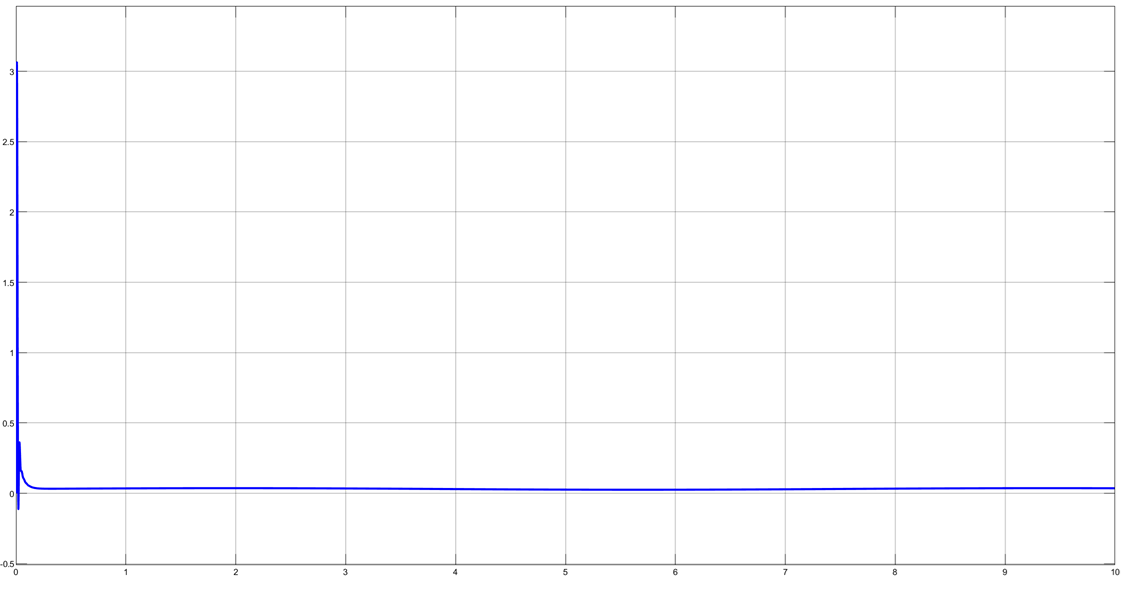
\includegraphics[width=0.88\textwidth,height=0.30\textheight,keepaspectratio]{imagenes/resultado_corriente.png}

\vspace{1mm}
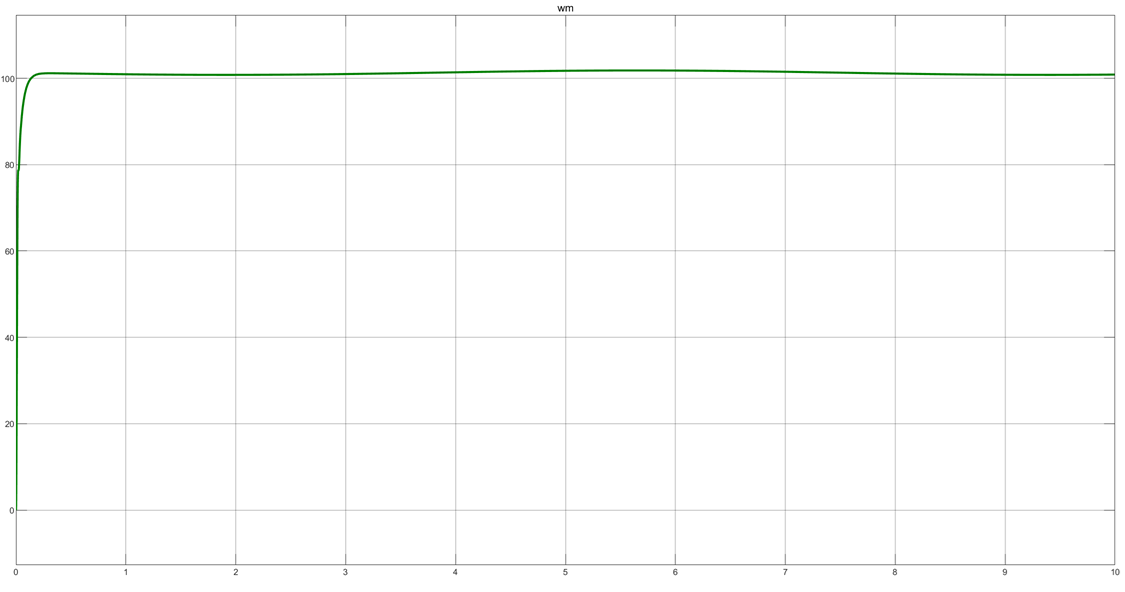
\includegraphics[width=0.88\textwidth,height=0.30\textheight,keepaspectratio]{imagenes/resultado_velocidad.png}

\vspace{2mm}
{\small \textbf{Interpretación física:} la corriente $i_q$ crece rápidamente por la dinámica inductiva y luego cae a medida que aparece la back-EMF. Ese torque acelera el rotor hasta que se equilibran torque motor y fricción viscosa.}
\end{frame}

\begin{frame}{Ensayo a lazo abierto: respuesta termica}
{\small\color{uncGray}La evolucion de temperatura confirma el acoplamiento correcto entre subsistema electrico, mecanico y termico dentro del modelo no lineal.}\par
\vspace{2mm}

\centering
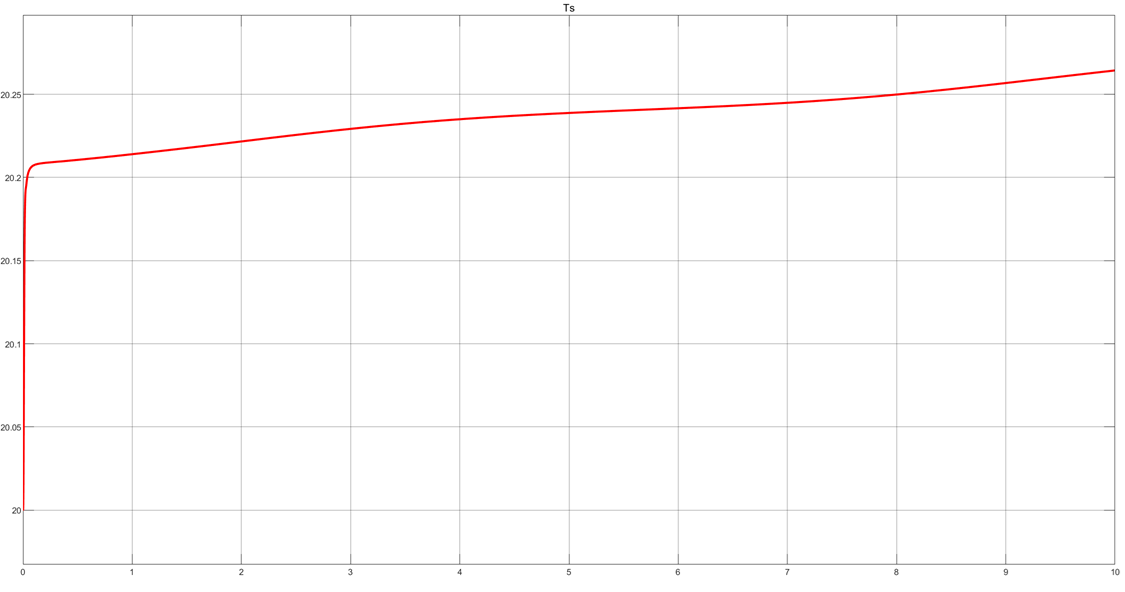
\includegraphics[width=0.90\textwidth,height=0.56\textheight,keepaspectratio]{imagenes/resultado_temperatura.png}

\vspace{2mm}
\begin{itemize}
  \item El estator parte en $T_s(0)=20^\circ$C y comienza a calentarse por perdidas Joule.
  \item La pendiente no es constante: es mayor al arranque, cuando la corriente es maxima y el rotor aun no desarrolla back-EMF significativa.
  \item Al aumentar la velocidad y disminuir la corriente, baja tambien la tasa de calentamiento.
\end{itemize}
\end{frame}

\subsection{Linealización del modelo no lineal}
\sectionslide{Linealización del modelo no lineal}

% -------------------------------------------------------------------
%  SLIDE 33 - Idea de linealizacion Jacobiana
% -------------------------------------------------------------------
\begin{frame}{Método de pequeñas señales: idea central}
{\small\color{uncGray}La primera linealización se realiza mediante el método de pequeñas señales: una expansión de Taylor de primer orden alrededor de un punto de operación cuasiestático.}\par
\vspace{3mm}

\textbf{Descomposicion en equilibrio + perturbacion:}
\begin{equation*}
\bm{x}(t)=\bm{x}_O+\Delta\bm{x}(t),
\qquad
\bm{u}(t)=\bm{u}_O+\Delta\bm{u}(t)
\end{equation*}

\textbf{Modelo no lineal de partida:}
\begin{equation*}
\dot{\bm{x}}=\bm{f}(\bm{x},\bm{u})
\end{equation*}

\textbf{Taylor de primer orden en $(\bm{x}_O,\bm{u}_O)$:}
\begin{equation*}
\Delta\dot{\bm{x}}(t)\approx
\underbrace{\left.\frac{\partial \bm{f}}{\partial \bm{x}}\right|_O}_{\bm{A}_O}
\Delta\bm{x}(t)+
\underbrace{\left.\frac{\partial \bm{f}}{\partial \bm{u}}\right|_O}_{\bm{B}_O}
\Delta\bm{u}(t)
\end{equation*}

{\small Resultado: un modelo \textbf{lineal local} válido para pequeñas variaciones respecto del equilibrio elegido.}
\end{frame}

% -------------------------------------------------------------------
%  SLIDE 34 - Punto de operacion
% -------------------------------------------------------------------
\begin{frame}{Punto de operación cuasiestático}
{\small\color{uncGray}El Jacobiano se evalúa en un estado de funcionamiento estacionario del sistema, definido por un conjunto de variables de operación constantes.}\par
\vspace{3mm}

\textbf{Condiciones clave del equilibrio:}
\begin{itemize}
  \item \textbf{Cinematica:} $\dot{\theta}_{mO}=\omega_{mO}$ con $\omega_{mO}$ constante.
  \item \textbf{Mecanica:} el torque electromagnetico compensa friccion, gravedad y carga:
  \[
  0=-b_{eq}\omega_{mO}+T_{mO}-g\,k_l\sin\!\big(\theta_{mO}/r\big)-T_{ldO}/r
  \]
  \item \textbf{Electrica:} las corrientes $i_{qsO}^r$, $i_{dsO}^r$ quedan fijadas por las tensiones de equilibrio $v_{qsO}^r$, $v_{dsO}^r$.
  \item \textbf{Termica:} la disipacion Joule iguala al intercambio con ambiente:
  \[
  0=\tfrac{3}{2}R_s(T_{sO}^\circ)\!\left(i_{qsO}^{r\,2}+i_{dsO}^{r\,2}\right)-\frac{T_{sO}^\circ-T_{ambO}^\circ}{R_{ts\text{-}amb}}
  \]
\end{itemize}

{\small Cada elección de $(\theta_{mO},\omega_{mO},i_{qsO}^r,i_{dsO}^r,T_{sO}^\circ)$ define un \textbf{modelo local distinto}.}
\end{frame}

% -------------------------------------------------------------------
%  SLIDE 35 - Modelo incremental LPV
% -------------------------------------------------------------------
\begin{frame}{Modelo incremental LPV}
{\small\color{uncGray}La linealización por pequeñas señales produce un sistema lineal en variables incrementales, pero con matrices que dependen del punto de operación: por eso el resultado es un modelo LPV.}\par
\vspace{3mm}

\textbf{Estado incremental reducido:}
\begin{equation*}
\Delta\bm{x}(t)=
\big[\,\Delta\theta_m,\;\Delta\omega_m,\;\Delta i_{qs}^{r},\;\Delta i_{ds}^{r},\;\Delta T_s^\circ\,\big]^T
\end{equation*}

\textbf{Entradas incrementales:}
\begin{equation*}
\Delta\bm{u}(t)=
\big[\,\Delta v_{qs}^{r},\;\Delta v_{ds}^{r},\;\Delta T_{ld},\;\Delta T_{amb}^\circ\,\big]^T
\end{equation*}

\textbf{Forma estructural:}
\begin{equation*}
\Delta\dot{\bm{x}}(t)=\bm{A}_O(\rho)\,\Delta\bm{x}(t)+\bm{B}_O(\rho)\,\Delta\bm{u}(t)
\end{equation*}

\textbf{Parámetros de operación} $\rho$:
\begin{equation*}
\rho=\big(\theta_{mO},\;\omega_{mO},\;i_{qsO}^{r},\;i_{dsO}^{r},\;T_{sO}^\circ\big)
\end{equation*}

{\small En otras palabras: la dinámica es lineal para perturbaciones pequeñas, pero \textbf{sus coeficientes cambian con el régimen de trabajo}.}
\end{frame}

% -------------------------------------------------------------------
%  SLIDE 36 - Estructura fisica de A0
% -------------------------------------------------------------------
\begin{frame}{Estructura física de las matrices LPV}
{\small\color{uncGray}No interesa memorizar la matriz completa, sino identificar qué fenómenos físicos quedan embebidos en sus coeficientes.}\par
\vspace{3mm}

\textbf{Terminos mas representativos del Jacobiano $\bm{A}_O$:}
\begin{equation*}
A_{21}=-\frac{g\,k_l}{J_{eq}\,r^2}\cos\!\left(\frac{\theta_{mO}}{r}\right)
\qquad
A_{32}=-\frac{P_p(\lambda'_m+L_d i_{dsO}^{r})}{L_q}
\end{equation*}
\begin{equation*}
A_{34}=-\frac{L_d P_p \omega_{mO}}{L_q}
\qquad
A_{43}=\frac{L_q P_p \omega_{mO}}{L_d}
\qquad
\frac{\partial \dot{i}_{qs}^{r}}{\partial T_s^\circ}\propto -\,R_{s,REF}\alpha_{Cu}\,i_{qsO}^{r}
\end{equation*}

\textbf{Lectura fisica:}
\begin{itemize}
  \item $A_{21}$ aporta una \textbf{rigidez gravitacional local} que depende de la posicion.
  \item $A_{32}$, $A_{34}$ y $A_{43}$ representan los \textbf{acoplamientos electromecanicos} entre velocidad y corrientes $q/d$.
  \item Los terminos en $T_s^\circ$ capturan la \textbf{variacion resistiva} del cobre con temperatura.
\end{itemize}

{\small Conclusión: el modelo LPV es \textbf{lineal local}, pero sigue reflejando gravedad, back-EMF, acoplamientos cruzados y efecto térmico. El paso siguiente será una \textbf{segunda linealización}, ahora por realimentación de no linealidades.}
\end{frame}

% -------------------------------------------------------------------
%  SLIDE 37 - Ley minima eje d
% -------------------------------------------------------------------
\begin{frame}{Segunda linealización: realimentación de no linealidades}
{\small\color{uncGray}Luego del modelo LPV, se aplica un segundo método de linealización: la realimentación de no linealidades. La idea es cancelar algebraicamente los acoplamientos internos mediante una ley de control sobre las entradas manipuladas.}\par
\vspace{3mm}

\textbf{Hipótesis de desacoplamiento:}
\begin{equation*}
i_{ds}^{r}(t)\equiv 0
\end{equation*}

\textbf{Ecuacion original del eje $d$:}
\begin{equation*}
\dot{i}_{ds}^{r}(t)=\frac{1}{L_d}\Big[\,v_{ds}^{r}(t)-R_{s0}i_{ds}^{r}(t)+L_q\,i_{qs}^{r}(t)\,\omega_r(t)\Big]
\end{equation*}

\textbf{Ley de control minima} para cancelar el acoplamiento cruzado:
\begin{equation*}
\boxed{\;v_{ds}^{r}(t)=-L_q\,i_{qs}^{r}(t)\,\omega_r(t)\;}
\end{equation*}

\textbf{Efecto fisico buscado:}
\begin{itemize}
  \item forzar $i_{ds}^{r}\to 0$,
  \item orientar el flujo sobre el eje de imanes,
  \item dejar el torque proporcional solo a $i_{qs}^{r}$.
\end{itemize}
\end{frame}

% -------------------------------------------------------------------
%  SLIDE 38 - Modelo LTI nominal
% -------------------------------------------------------------------
\begin{frame}{Modelo LTI nominal resultante}
{\small\color{uncGray}Aplicando la ley mínima en el eje $d$ y fijando $R_s=R_{s0}$ constante, la planta electromecánica principal queda reducida a tres estados dinámicos.}\par
\vspace{2mm}

\footnotesize
\begin{equation*}
\left\{
\begin{aligned}
\dot{\theta}_m &= \omega_m \\[2pt]
\dot{\omega}_m &= \frac{1}{J_{eq}}\!\left[\frac{3}{2}P_p\lambda'_m\,i_{qs}-b_{eq}\omega_m-\frac{1}{r}T_{ld}-\frac{g\,k_l}{r}\sin\!\left(\frac{\theta_m}{r}\right)\right] \\[4pt]
\dot{i}_{qs} &= \frac{1}{L_q}\!\left[-P_p\lambda'_m\,\omega_m-R_{s0}i_{qs}+v_{qs}\right]
\end{aligned}
\right.
\end{equation*}
\normalsize

\textbf{Estado nominal:}
\begin{equation*}
\bm{x}_{LTI}(t)=\big[\,\theta_m,\;\omega_m,\;i_{qs}\,\big]^T
\end{equation*}

\textbf{Observación importante:}
\begin{itemize}
  \item La temperatura del estator sigue calculándose en simulación.
  \item Pero la \textbf{dinámica principal} del modelo nominal queda concentrada en la terna $(\theta_m,\omega_m,i_{qs})$.
\end{itemize}
\end{frame}

% -------------------------------------------------------------------
%  SLIDE 39 - Forma matricial e interpretacion
% -------------------------------------------------------------------
\begin{frame}{Forma matricial e interpretación física}
{\small\color{uncGray}La representación matricial hace explícito que el control actúa por $v_{qs}$, mientras que carga y gravedad ingresan como perturbaciones mecánicas.}\par
\vspace{2mm}

\centering
\resizebox{\textwidth}{!}{$
\dot{\bm{x}}_{LTI}=
\underbrace{\begin{bmatrix}
0 & 1 & 0\\
0 & -\frac{b_{eq}}{J_{eq}} & \frac{3P_p\lambda'_m}{2J_{eq}}\\
0 & -\frac{P_p\lambda'_m}{L_q} & -\frac{R_{s0}}{L_q}
\end{bmatrix}}_{\bm{A}}
\bm{x}_{LTI}+
\underbrace{\begin{bmatrix}0\\0\\ \frac{1}{L_q}\end{bmatrix}}_{\bm{B}_c}v_{qs}
+
\underbrace{\begin{bmatrix}0\\-\frac{1}{rJ_{eq}}\\0\end{bmatrix}}_{\bm{B}_{d1}}T_{ld}
+
\underbrace{\begin{bmatrix}0\\-\frac{g\,k_l}{rJ_{eq}}\\0\end{bmatrix}}_{\bm{B}_{d2}}
\sin\!\left(\frac{\theta_m}{r}\right)
$}

\textbf{Interpretación del modelo:}
\begin{itemize}
  \item $\bm{A}$ contiene la planta electromecánica nominal.
  \item $\bm{B}_c$ muestra que la acción de control entra solo por el canal de corriente $q$.
  \item $\bm{B}_{d1}$ y $\bm{B}_{d2}$ separan la carga aplicada y el torque gravitacional.
\end{itemize}

{\small Esta separación es la base para el análisis posterior de estabilidad, funciones de transferencia y desempeño del controlador.}
\end{frame}

% -------------------------------------------------------------------
%  SLIDE 40 - Diagrama del LTI nominal
% -------------------------------------------------------------------
\figslide{Diagrama del modelo LTI nominal}{%
El diagrama resume la estructura final del modelo nominal: la corriente $i_{qs}$ genera torque, la velocidad realimenta por back-EMF y las perturbaciones mecánicas ingresan por canales separados. Sobre esta planta se apoyarán el modelo aumentado y los análisis posteriores a lazo abierto.%
}{LTI equivalente_nominal.png}

\subsection{Modelo LTI aumentado e implementación}
\sectionslide{Modelo LTI aumentado e implementación}

% -------------------------------------------------------------------
%  SLIDE 44 - Dinamica residual
% -------------------------------------------------------------------
\begin{frame}{Dinámica residual del eje $d$}
{\small\color{uncGray}El modelo nominal supone $i_{ds}^r(0)=0$. Si esa condición inicial no se cumple, aparece una dinámica residual propia del eje directo, aun cuando se aplique la ley mínima de desacoplamiento.}\par
\vspace{3mm}

\textbf{Con la ley minima} $v_{ds}^{r}=-L_q i_{qs}^{r}\omega_r$:
\begin{equation*}
\dot{i}_{ds}^{r}(t)= -\frac{R_{s0}}{L_d}\,i_{ds}^{r}(t)
\end{equation*}

\textbf{Solucion temporal:}
\begin{equation*}
i_{ds}^{r}(t)=i_{ds}^{r}(0)\,e^{-\frac{R_{s0}}{L_d}t}
\end{equation*}

\textbf{Interpretacion fisica:}
\begin{itemize}
  \item $i_{ds}^{r}$ no diverge ni excita modos adicionales acoplados.
  \item Decae exponencialmente hacia cero con constante de tiempo
  \[
  \tau_d=\frac{L_d}{R_{s0}}
  \]
  \item Esa dinámica residual es transitoria, pero conviene incorporarla al modelo para cubrir el caso general $i_{ds}^r(0)\neq 0$.
\end{itemize}
\end{frame}

% -------------------------------------------------------------------
%  SLIDE 45 - Ley complementaria eje q
% -------------------------------------------------------------------
\begin{frame}{Ley complementaria en el eje $q$}
{\small\color{uncGray}Aunque $i_{ds}^{r}$ decae por sí sola, mientras no sea exactamente nula vuelve a introducir acoplamiento cruzado en la ecuación del eje $q$. La solución es compensarlo en línea.}\par
\vspace{3mm}

\textbf{Acoplamiento residual sobre el eje $q$:}
\begin{equation*}
v_{qs}^{r}(t)=L_q\dot{i}_{qs}^{r}(t)+R_s i_{qs}^{r}(t)+\lambda'_m\omega_r(t)+
\underbrace{\omega_r(t)L_d i_{ds}^{r}(t)}_{\text{acoplamiento cruzado}}
\end{equation*}

\textbf{Ley de control complementaria:}
\begin{equation*}
\boxed{\;v_{qs}^{r*}(t)=v_{qs}(t)+\omega_r(t)L_d i_{ds}^{r}(t)\;}
\end{equation*}

\textbf{Resultado buscado:}
\begin{itemize}
  \item cancelar el termino cruzado restante,
  \item conservar $v_{qs}(t)$ como nueva entrada lineal de control,
  \item obtener un modelo equivalente valido tambien para $i_{ds}^{r}(0)\neq 0$.
\end{itemize}
\end{frame}

% -------------------------------------------------------------------
%  SLIDE 46 - Modelo LTI aumentado escalar
% -------------------------------------------------------------------
\begin{frame}{Modelo LTI aumentado de cuarto orden}
{\small\color{uncGray}Incorporando la dinámica residual de $i_{ds}^{r}$ y la ley complementaria en el eje $q$, el modelo lineal equivalente queda ampliado a cuatro estados.}\par
\vspace{2mm}

\textbf{Estado aumentado:}
\begin{equation*}
\bm{x}_{aug}(t)=\big[\,\theta_m,\;\omega_m,\;i_{qs},\;i_{ds}^{r}\,\big]^T
\end{equation*}

\footnotesize
\begin{equation*}
\left\{
\begin{aligned}
\dot{\theta}_m &= \omega_m \\[2pt]
\dot{\omega}_m &= \frac{1}{J_{eq}}\!\left[\frac{3}{2}P_p\lambda'_m\,i_{qs}-b_{eq}\omega_m-\frac{1}{r}T_{ld}-\frac{g\,k_l}{r}\sin\!\left(\frac{\theta_m}{r}\right)\right] \\[4pt]
\dot{i}_{qs} &= \frac{1}{L_q}\!\left[-P_p\lambda'_m\,\omega_m-R_{s0}i_{qs}+v_{qs}\right] \\[4pt]
\dot{i}_{ds}^{r} &= -\frac{R_{s0}}{L_d}\,i_{ds}^{r}
\end{aligned}
\right.
\end{equation*}
\normalsize

{\small La temperatura puede seguir simulándose aparte, pero la dinámica electromecánica lineal equivalente queda contenida en estos cuatro estados.}
\end{frame}

% -------------------------------------------------------------------
%  SLIDE 47 - Forma matricial aumentado
% -------------------------------------------------------------------
\begin{frame}{Forma matricial del modelo aumentado}
{\small\color{uncGray}La estructura matricial deja ver que $i_{ds}^{r}$ evoluciona como un modo desacoplado de primer orden, mientras la terna $(\theta_m,\omega_m,i_{qs})$ conserva la misma planta nominal.}\par
\vspace{2mm}

\centering
\resizebox{\textwidth}{!}{$
\dot{\bm{x}}_{aug}=
\underbrace{\begin{bmatrix}
0 & 1 & 0 & 0\\
0 & -\frac{b_{eq}}{J_{eq}} & \frac{3P_p\lambda'_m}{2J_{eq}} & 0\\
0 & -\frac{P_p\lambda'_m}{L_q} & -\frac{R_{s0}}{L_q} & 0\\
0 & 0 & 0 & -\frac{R_{s0}}{L_d}
\end{bmatrix}}_{\bm{A}_{aug}}
\bm{x}_{aug}+
\underbrace{\begin{bmatrix}0\\0\\ \frac{1}{L_q}\\0\end{bmatrix}}_{\bm{B}_c}v_{qs}
+
\underbrace{\begin{bmatrix}0\\-\frac{1}{rJ_{eq}}\\0\\0\end{bmatrix}}_{\bm{B}_{d1}}T_{ld}
+
\underbrace{\begin{bmatrix}0\\-\frac{g\,k_l}{rJ_{eq}}\\0\\0\end{bmatrix}}_{\bm{B}_{d2}}
\sin\!\left(\frac{\theta_m}{r}\right)
$}

\textbf{Interpretación del modelo:}
\begin{itemize}
  \item el cuarto estado no realimenta a la dinámica nominal,
  \item pero queda explícitamente representado para cubrir condiciones iniciales no nulas,
  \item así el modelo sigue siendo útil para análisis y simulación comparativa.
\end{itemize}
\end{frame}

% -------------------------------------------------------------------
%  SLIDE 48 - Diagrama aumentado
% -------------------------------------------------------------------
\figslide{Diagrama del modelo LTI aumentado}{%
El diagrama de bloques muestra la extensión natural del modelo nominal: se conserva la cadena mecánica principal y se agrega el modo residual de $i_{ds}^{r}$, ya desacoplado del eje $q$ por la ley complementaria.%
}{LTI equivalente_aumentado.png}

% -------------------------------------------------------------------
%  SLIDE 49 - Implementacion sobre la planta NL
% -------------------------------------------------------------------
\figslide{Implementación sobre la planta no lineal}{%
La linealización por realimentación no se aplica sobre una planta abstracta, sino como un controlador parcial acoplado a la planta NL: recibe $v_{qs}$, estima variables internas, calcula $v_{qs}^{r*}$ y $v_{ds}^{r*}$, y luego excita físicamente al inversor mediante la Park inversa.%
}{NL con realimentacion NL.png}

% -------------------------------------------------------------------
%  SLIDE 50 - Flujo de implementacion
% -------------------------------------------------------------------
\begin{frame}{Flujo de implementación de la realimentación NL}
{\small\color{uncGray}La realización física del modelo equivalente exige calcular en tiempo real las tensiones virtuales de desacoplamiento a partir de mediciones idealizadas de corriente y velocidad.}\par
\vspace{3mm}

\begin{enumerate}
  \item El controlador externo genera la accion lineal $v_{qs}(t)$.
  \item Las corrientes medidas $\bm{i}_{abc}$ se transforman a $\bm{i}_{qd0}^{r}$ mediante Park directa.
  \item Con $\omega_m(t)$ e $i_{ds}^{r}(t)$ se calculan:
  \[
  v_{ds}^{r*}(t)=-L_q i_{qs}^{r}(t)\omega_r(t),
  \qquad
  v_{qs}^{r*}(t)=v_{qs}(t)+\omega_r(t)L_d i_{ds}^{r}(t)
  \]
  \item Las referencias $v_{qd}^{r*}$ vuelven al marco trifasico por Park inversa y alimentan al inversor.
\end{enumerate}

{\small En resumen: la linealización equivalente se obtiene \textbf{por realimentación no lineal}, calculando tensiones de compensación sin modificar la planta física.}
\end{frame}

% -------------------------------------------------------------------
%  SLIDE 51 - Comparacion conceptual
% -------------------------------------------------------------------
\begin{frame}{LPV vs. LTI aumentado: comparación conceptual}
{\small\color{uncGray}Ambos modelos son lineales en su forma final, pero no representan la misma idea de linealización ni tratan igual las no linealidades físicas del accionamiento.}\par
\vspace{3mm}

\textbf{Modelo LPV por pequeñas señales}
\begin{itemize}
  \item surge de un Jacobiano local,
  \item depende del punto de operación $(\theta_{mO},\omega_{mO},i_{qsO}^{r},i_{dsO}^{r},T_{sO}^\circ)$,
  \item incorpora la gravedad linealizada como una rigidez local.
\end{itemize}

\textbf{Modelo LTI aumentado por realimentación NL}
\begin{itemize}
  \item surge de cancelar algebraicamente no linealidades internas,
  \item mantiene la matriz de estado invariante,
  \item extrae la gravedad como perturbación externa y desacopla el eje $d$.
\end{itemize}

{\small Si se fuerza $i_{dsO}^{r}\equiv 0$, el LPV se acerca estructuralmente al LTI aumentado; por eso ambos modelos son comparables, pero no equivalentes en su origen.}
\end{frame}

% -------------------------------------------------------------------
%  SLIDE 52 - Variaciones de ids y funciones de transferencia
% -------------------------------------------------------------------
\subsection{Variaciones de corriente en eje d y funciones de transferencia}
\sectionslide{Variaciones de $i_{ds}^{r}$ y funciones de transferencia}

% -------------------------------------------------------------------
%  SLIDE 53 - ids como parametro
% -------------------------------------------------------------------
\begin{frame}{Corriente de eje $d$ como parámetro}
{\small\color{uncGray}Al liberar la condición $I_{dsO}^{r}=0$, la corriente directa deja de ser solo un estado residual y pasa a modificar la capacidad estática de torque y la dinámica local del modelo LPV.}\par
\vspace{3mm}

\textbf{Torque electromagnético en operación estacionaria:}
\begin{equation*}
T_m=\frac{3}{2}P_p\Big[\lambda'_m+(L_d-L_q)I_{dsO}^{r}\Big]I_{qsO}^{r}
\end{equation*}

\textbf{Qué cambia respecto del caso base:}
\begin{itemize}
  \item Con $I_{dsO}^{r}=0$, el torque queda asociado al flujo de los imanes y a $I_{qsO}^{r}$.
  \item Con $I_{dsO}^{r}\neq 0$, aparece el aporte de reluctancia por saliencia.
  \item El mismo parámetro desplaza los autovalores del Jacobiano LPV.
\end{itemize}

{\small Esta es una lectura local del LPV: no reemplaza al LTI aumentado, sino que muestra cómo cambia el modelo alrededor de otros puntos de operación.}
\end{frame}

% -------------------------------------------------------------------
%  SLIDE 54 - Reforzamiento y debilitamiento
% -------------------------------------------------------------------
\begin{frame}{Reforzamiento y debilitamiento de campo}
{\small\color{uncGray}La inyección de corriente en eje $d$ altera el flujo magnético total. Según el signo, puede priorizar torque por amperio o margen de tensión a alta velocidad.}\par
\vspace{2mm}

\begin{columns}[T,onlytextwidth]
\column{0.42\textwidth}
\centering
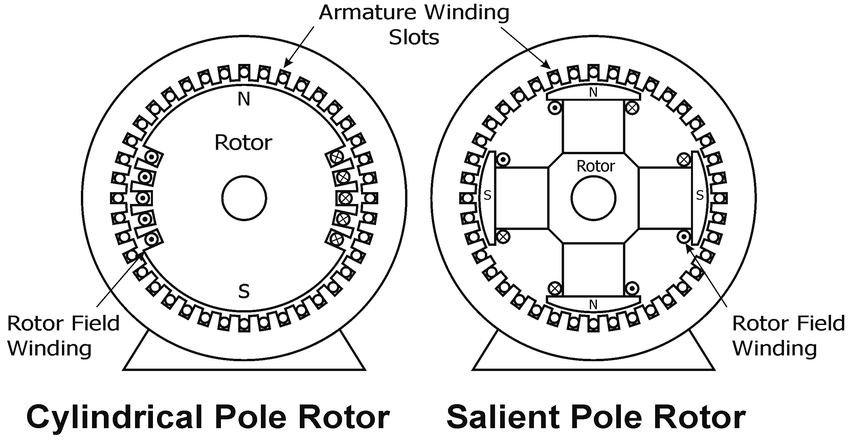
\includegraphics[width=\linewidth]{imagenes/polosaliente_cilindrico.png}

\column{0.54\textwidth}
\textbf{Dos regímenes de operación:}
\begin{itemize}
  \item \textbf{$I_{dsO}^{r}>0$:} reforzamiento de campo. Aumenta el flujo efectivo y puede sumar torque de reluctancia si $L_d>L_q$.
  \item \textbf{$I_{dsO}^{r}<0$:} debilitamiento de campo. Reduce el flujo efectivo y la fuerza contraelectromotriz.
  \item El costo del debilitamiento es menor torque para el mismo $I_{qsO}^{r}$; el beneficio es mayor velocidad antes de saturar tensión.
\end{itemize}
\end{columns}
\end{frame}

% -------------------------------------------------------------------
%  SLIDE 55 - Migracion con ids
% -------------------------------------------------------------------
\begin{frame}{Migración dinámica con $I_{dsO}^{r}$}
{\small\color{uncGray}El barrido de $I_{dsO}^{r}$ permite ver cómo cambian los autovalores del Jacobiano LPV entre debilitamiento y reforzamiento de campo.}\par
\vspace{1mm}

\centering

\includegraphics[width=0.88\textwidth,height=0.52\textheight,keepaspectratio]{imagenes/migracion_ids_2.png}

\vspace{1mm}
\raggedright
\textbf{Resultado principal:}\;
{\small
\begin{itemize}
  \item Al aumentar $I_{dsO}^{r}$, aumenta la frecuencia de oscilación de los polos dominantes.
  \item La parte real se mantiene casi constante: no se degrada severamente la estabilidad local.
  \item Los modos rápido eléctrico y térmico quedan prácticamente invariantes.
\end{itemize}
}
\end{frame}

% -------------------------------------------------------------------
%  SLIDE 56 - Planteo de funciones de transferencia
% -------------------------------------------------------------------
\begin{frame}{Funciones de transferencia del LTI aumentado}
{\small\color{uncGray}A partir del modelo LTI aumentado se buscan las relaciones entrada-salida desde $v_{qs}$ y $T_{ld}$ hacia la posición $\theta_m$.}\par
\vspace{3mm}

\textbf{Condiciones usadas para obtenerlas:}
\begin{itemize}
  \item Modelo incremental con $\bm{x}_{aug}(0)=\bm{0}$.
  \item Resistencia constante: $R_s=R_{s0}$.
  \item La gravedad se trata como perturbación externa compensable, no como parte de la matriz $\bm{A}_{aug}$.
  \item Como $i_{ds}^{r}$ queda desacoplado, la relación entrada-salida se obtiene con el subsistema nominal de tercer orden.
\end{itemize}

\begin{equation*}
G(s)=\bm{C}\,(s\bm{I}-\bm{A})^{-1}\bm{B}
\end{equation*}
\end{frame}

% -------------------------------------------------------------------
%  SLIDE 57 - Funciones de transferencia finales
% -------------------------------------------------------------------
\begin{frame}{Funciones de transferencia obtenidas}
{\small\color{uncGray}Ambas funciones comparten el mismo denominador de tercer orden. El factor asociado a $i_{ds}^{r}$ no aparece en la relación entrada-salida.}\par
\vspace{2mm}

\small
\begin{equation*}
\Delta_3(s)=
s^3+
\left(\frac{b_{eq}}{J_{eq}}+\frac{R_{s0}}{L_q}\right)s^2+
\left(\frac{b_{eq}R_{s0}}{J_{eq}L_q}+
\frac{3P_p^2{\lambda'_m}^{\,2}}{2J_{eq}L_q}\right)s
\end{equation*}

\vspace{2mm}
\resizebox{\textwidth}{!}{$
G_1(s)=\frac{\theta_m(s)}{v_{qs}(s)}
=
\frac{\dfrac{3P_p\lambda'_m}{2J_{eq}L_q}}{\Delta_3(s)}
\qquad\qquad
G_2(s)=\frac{\theta_m(s)}{T_{ld}(s)}
=
\frac{-\dfrac{1}{rJ_{eq}}\left(s+\dfrac{R_{s0}}{L_q}\right)}{\Delta_3(s)}
$}
\normalsize

\vspace{3mm}
\textbf{Interpretación:}
\begin{itemize}
  \item $G_1$ no tiene ceros finitos.
  \item $G_2$ posee un cero en $s=-R_{s0}/L_q$ asociado al canal eléctrico de perturbación.
\end{itemize}
\end{frame}

% -------------------------------------------------------------------
%  SLIDE 58 - Estado oculto
% -------------------------------------------------------------------
\begin{frame}{Estado interno fuera de las funciones de transferencia}
{\small\color{uncGray}El cuarto estado del modelo aumentado aparece en espacio de estados, pero no se refleja en las funciones de transferencia hacia $\theta_m$.}\par
\vspace{3mm}

\begin{columns}[T,onlytextwidth]
\column{0.45\textwidth}
\textbf{Modo residual:}
\begin{equation*}
\lambda_d=-\frac{R_{s0}}{L_d}
\end{equation*}
\begin{equation*}
i_{ds}^{r}(t)=i_{ds}^{r}(0)e^{-\frac{R_{s0}}{L_d}t}
\end{equation*}

\column{0.51\textwidth}
\textbf{Por qué no aparece:}
\begin{itemize}
  \item $v_{qs}$ y $T_{ld}$ no excitan directamente a $i_{ds}^{r}$.
  \item La salida $\theta_m$ no depende de $i_{ds}^{r}$.
  \item La cuarta fila de $\bm{A}_{aug}$ queda desacoplada del resto del sistema.
\end{itemize}
\end{columns}

\vspace{2mm}
{\small En consecuencia, el polo de $i_{ds}^{r}$ se cancela al pasar de espacio de estados a funciones de transferencia.}
\end{frame}

% -------------------------------------------------------------------
%  SLIDE 59 - Estabilidad a lazo abierto
% -------------------------------------------------------------------
\begin{frame}{Autovalores y estabilidad a lazo abierto}
{\small\color{uncGray}El polinomio característico del modelo aumentado separa el integrador de posición, el modo electromecánico y el modo residual del eje $d$.}\par
\vspace{2mm}

\begin{equation*}
\det(s\bm{I}-\bm{A}_{aug})=
\underbrace{\left(s+\frac{R_{s0}}{L_d}\right)}_{\lambda_4}
\underbrace{s}_{\lambda_1}
\underbrace{\left(s^2+a_2s+a_1\right)}_{\lambda_{2,3}}
\end{equation*}

\textbf{Valores nominales:}
\begin{itemize}
  \item $\lambda_1=0$: integrador cinemático de posición.
  \item $\lambda_{2,3}=-91{,}7\pm j\,148{,}0$: modo electromecánico subamortiguado, $\zeta\simeq0{,}527$.
  \item $\lambda_4=-160{,}3$: dinámica residual de $i_{ds}^{r}$, con $\tau_d\simeq6{,}24$ ms.
\end{itemize}

\textbf{Conclusión:}
{\small el sistema es marginalmente estable internamente, pero no BIBO estable desde $v_{qs}$ o $T_{ld}$ hacia $\theta_m$ por el polo en el origen.}
\end{frame}

% -------------------------------------------------------------------
%  SLIDE 60 - Mapa polos y ceros
% -------------------------------------------------------------------
\figslide{Mapa de polos y ceros a lazo abierto}{%
El mapa confirma la estructura anterior: un polo en el origen, el par electromecánico complejo y el polo residual de $i_{ds}^{r}$ marcado como cancelado. Esta lectura justifica que el diseño posterior cierre el lazo de posición y trate a la carga como perturbación.% 
}{polos_ceros_LA.png}

% -------------------------------------------------------------------
%  SLIDE 61 - Variaciones parametricas
% -------------------------------------------------------------------
\subsection{Variaciones paramétricas y propiedades estructurales}
\sectionslide{Variaciones paramétricas y propiedades estructurales}

% -------------------------------------------------------------------
%  SLIDE 62 - Variacion de Rs
% -------------------------------------------------------------------
\begin{frame}{Migración ante variación de $R_s$}
{\small\color{uncGray}La resistencia del estator cambia con la temperatura. En el LTI aumentado, su variación desplaza el amortiguamiento y el cero de perturbación, pero casi no altera la frecuencia natural.}\par
\vspace{2mm}

\begin{columns}[T,onlytextwidth]
\column{0.60\textwidth}
\centering

\includegraphics[width=\linewidth]{imagenes/migracion_Rs.png}

\column{0.37\textwidth}
\textbf{Lectura física:}
\begin{itemize}
  \item $\omega_n$ permanece cerca de $174$ rad/s.
  \item $\zeta$ aumenta con $R_s$: hay mayor disipación eléctrica.
  \item El cero de $G_2$ migra como $z=-R_s/L_q$.
\end{itemize}
\end{columns}
\end{frame}

% -------------------------------------------------------------------
%  SLIDE 63 - Variacion de carga
% -------------------------------------------------------------------
\begin{frame}{Migración ante variación de carga}
{\small\color{uncGray}La masa de carga modifica la inercia equivalente $J_{eq}$ y, con ello, el modo electromecánico dominante del sistema.}\par
\vspace{2mm}

\begin{columns}[T,onlytextwidth]
\column{0.60\textwidth}
\centering

\includegraphics[width=\linewidth]{imagenes/migracion_ml.png}

\column{0.37\textwidth}
\textbf{Efecto observado:}
\begin{itemize}
  \item Al aumentar $m_l$, crece la inercia equivalente.
  \item La frecuencia natural disminuye.
  \item El amortiguamiento relativo aumenta.
  \item El polo en el origen y el cero de $G_2$ permanecen invariantes.
\end{itemize}
\end{columns}

{\small Estas variaciones anticipan la necesidad de un controlador robusto frente al rango de carga.}
\end{frame}

% -------------------------------------------------------------------
%  SLIDE 64 - Bode a lazo abierto
% -------------------------------------------------------------------
\figslide{Bode a lazo abierto del LTI aumentado}{%
Los diagramas muestran la respuesta en frecuencia de los canales $G_1(s)=\theta_m/v_{qs}$ y $G_2(s)=\theta_m/T_{ld}$. La pendiente de baja frecuencia refleja el integrador de posición, mientras que el modo electromecánico domina la zona dinámica relevante para el diseño posterior.% 
}{bode_LA.png}

% -------------------------------------------------------------------
%  SLIDE 65 - Observabilidad y controlabilidad
% -------------------------------------------------------------------
\subsection{Observabilidad y controlabilidad}
\begin{frame}{Propiedades estructurales del modelo aumentado}
{\small\color{uncGray}Después de obtener las funciones de transferencia, conviene volver al espacio de estados para identificar qué estados se pueden observar y controlar con las señales disponibles.}\par
\vspace{3mm}

\textbf{Pregunta de observabilidad:}
\begin{itemize}
  \item ¿Puede reconstruirse $\bm{x}_{aug}$ midiendo solo $\theta_m$ o solo $\omega_m$?
\end{itemize}

\textbf{Pregunta de controlabilidad:}
\begin{itemize}
  \item ¿Puede actuarse sobre todos los estados usando solo $v_{qs}$?
\end{itemize}

\textbf{Idea clave:}
{\small el estado $i_{ds}^{r}$ ya apareció como modo desacoplado; ahora se formaliza esa lectura con rangos de matrices.}
\end{frame}

% -------------------------------------------------------------------
%  SLIDE 66 - Observabilidad desde theta
% -------------------------------------------------------------------
\begin{frame}{Observabilidad desde posición}
{\small\color{uncGray}Con un sensor de posición, la salida elegida es $\bm{C}_\theta=[\,1\;0\;0\;0\,]$. La cadena cinemática permite recuperar información de velocidad y corriente de eje $q$.}\par
\vspace{3mm}

\begin{equation*}
\mathcal{O}_\theta=
\begin{bmatrix}
\bm{C}_\theta\\
\bm{C}_\theta\bm{A}\\
\bm{C}_\theta\bm{A}^2\\
\bm{C}_\theta\bm{A}^3
\end{bmatrix},
\qquad
\operatorname{rango}(\mathcal{O}_\theta)=3<4
\end{equation*}

\textbf{Resultado:}
\begin{itemize}
  \item $\theta_m$ se mide directamente.
  \item $\omega_m$ aparece como derivada de $\theta_m$.
  \item $i_{qs}$ se manifiesta por el acoplamiento electromecánico.
  \item $i_{ds}^{r}$ no aparece: no acopla con la salida.
\end{itemize}
\end{frame}

% -------------------------------------------------------------------
%  SLIDE 67 - Observabilidad desde velocidad
% -------------------------------------------------------------------
\begin{frame}{Observabilidad desde velocidad}
{\small\color{uncGray}Si se mide solo velocidad, la salida pasa a ser $\bm{C}_\omega=[\,0\;1\;0\;0\,]$. Esta medición pierde información estructural respecto del sensor de posición.}\par
\vspace{3mm}

\begin{equation*}
\mathcal{O}_\omega=
\begin{bmatrix}
\bm{C}_\omega\\
\bm{C}_\omega\bm{A}\\
\bm{C}_\omega\bm{A}^2\\
\bm{C}_\omega\bm{A}^3
\end{bmatrix},
\qquad
\operatorname{rango}(\mathcal{O}_\omega)=2<4
\end{equation*}

\textbf{Estados no observables:}
\begin{itemize}
  \item $\theta_m$: la velocidad no contiene la condición inicial de posición.
  \item $i_{ds}^{r}$: sigue siendo un modo interno desacoplado.
\end{itemize}

{\small Por eso, para este sistema el sensor de posición es más informativo que medir solo velocidad.}
\end{frame}

% -------------------------------------------------------------------
%  SLIDE 68 - Controlabilidad desde vqs
% -------------------------------------------------------------------
\begin{frame}{Controlabilidad desde $v_{qs}$}
{\small\color{uncGray}La entrada lineal de control actúa directamente sobre la corriente de eje $q$ y desde allí se propaga hacia la velocidad y la posición.}\par
\vspace{3mm}

\begin{equation*}
\mathcal{C}_{v_q}=
\begin{bmatrix}
\bm{B}_c & \bm{A}\bm{B}_c & \bm{A}^2\bm{B}_c & \bm{A}^3\bm{B}_c
\end{bmatrix},
\qquad
\operatorname{rango}(\mathcal{C}_{v_q})=3<4
\end{equation*}

\textbf{Cadena controlable:}
\begin{equation*}
v_{qs}\;\longrightarrow\;i_{qs}\;\longrightarrow\;\omega_m\;\longrightarrow\;\theta_m
\end{equation*}

\textbf{Estado no controlable desde $v_{qs}$:}
\begin{itemize}
  \item $i_{ds}^{r}$, porque la cuarta fila queda desacoplada y $B_c(4)=0$.
\end{itemize}
\end{frame}

% -------------------------------------------------------------------
%  SLIDE 69 - Entrada adicional vds
% -------------------------------------------------------------------
\begin{frame}{Entrada adicional en eje $d$}
{\small\color{uncGray}El estado $i_{ds}^{r}$ podría controlarse agregando la tensión de eje directo como segunda entrada manipulable.}\par
\vspace{2mm}

\begin{equation*}
\bm{B}_{ext}=
\begin{bmatrix}
0 & 0\\
0 & 0\\
\frac{1}{L_q} & 0\\
0 & \frac{1}{L_d}
\end{bmatrix},
\qquad
\operatorname{rango}(\mathcal{C}_{ext})=4
\end{equation*}

\textbf{Interpretación:}
\begin{itemize}
  \item Matemáticamente, $v_{ds}^{r}$ completa la controlabilidad del modelo aumentado.
  \item En la estrategia adoptada, esa tensión ya se usa por la ley mínima para forzar $i_{ds}^{r}\to0$.
  \item No se trata de un grado de libertad libre para el control externo de posición.
\end{itemize}
\end{frame}

% -------------------------------------------------------------------
%  SLIDE 70 - Resumen estructural
% -------------------------------------------------------------------
\begin{frame}{Resumen estructural del LTI aumentado}
{\small\color{uncGray}Las funciones de transferencia y los rangos de observabilidad/controlabilidad llevan a la misma conclusión: el eje $d$ queda como modo interno oculto.}\par
\vspace{3mm}

\centering
\small
\begin{tabular}{lcccc}
\toprule
\textbf{Estado} & \textbf{Controlable} & \textbf{Obs. desde $\theta_m$} & \textbf{Obs. desde $\omega_m$} & \textbf{En FTs}\\
\midrule
$\theta_m$ & Sí & Sí & No & Sí\\
$\omega_m$ & Sí & Sí & Sí & Sí\\
$i_{qs}$ & Sí & Sí & Sí & Sí\\
$i_{ds}^{r}$ & No & No & No & No\\
\bottomrule
\end{tabular}
\normalsize

\vspace{4mm}
\raggedright
{\small Esta propiedad justifica usar el modelo nominal de tercer orden para la relación entrada-salida y conservar el cuarto estado solo para representar condiciones iniciales no nulas.}
\end{frame}


\end{document}
